\jrnlday{Les cieux déclarent Sa gloire}


\dvepigraph{%
Jésus était né à Bethléhem en Judée, au temps du roi Hérode. Des mages d’Orient arrivèrent à Jérusalem et dirent≡ Où est le roi des Juifs qui vient de naître? Car nous avons vu son étoile en Orient, et nous sommes venus l’adorer.}{\ibibleverse{Mt}(2:1,2)}

Dieu a utilisé les cieux et la terre pour proclamer la naissance glorieuse de Son Fils. Il a réuni une étoile, des planètes, une variété étrange de personnes et même des anges, tout cela dans un seul but≡ annoncer la naissance étonnante du Roi des rois - Jésus-Christ - Le Sauveur du monde.

L'un des signes les plus étonnants de ce premier Noël, c'est l'étoile de Bethléhem que les mages ont vue en Orient et qui les a dirigés pour venir adorer Jésus. Nous ne savons pas vraiment ce qu'était cette brillante étoile de Noël, mais beaucoup se sont livrés à des spéculations≡ certains optent pour une comète, d'autres pour une supernova, d'autres encore pensent que c'était la présence de la \emph{Shékinah}, la Gloire de Dieu, brillant des cieux pour éclairer l'endroit où Jésus est né.

Johannes Kepler, le fondateur de l'astronomie moderne, et un contemporain de Galilée, a mis en avance une théorie intéressante. L'un de ses étudiants appelé Jan Brunowski observait les cieux la nuit du 17 Décembre 1603 quand il nota qu'une remarquable conjonction s'était produite entre Saturne et Jupiter. Cette conjonction s'est poursuivie jusqu'en 1604, et au printemps de cette année-là, Mars a rejoint Saturne et Jupiter dans une triple conjonction. Quand cette conjonction est arrivée, une lumière comme celle d'une étoile de très forte magnitude est apparue et a continué à briller toute une année, puis elle a progressivement décrue avant de finir par disparaître. Brunowski l'a décrite comme \og étincelant d'une succession de couleurs comme un diamant \fg{}.

Kepler, qui était aussi un spécialiste érudit de la Bible, a pensé aux Mages et s'est demandé si ce phénomène ne s'était pas aussi produit au moment de la naissance de Jésus. Après une étude très complète, Kepler a découvert qu'une conjonction de Jupiter, Saturne et Mars arrive une fois tous les huit cents ans. En remontant dans le temps pour calculer la date, il a trouvé que cette conjonction s'était produite exactement deux ans avant la mort d'Hérode le Grand.

Nous ne savons pas de façon certaine si c'est de cette façon que l'étoile de Bethléhem est apparue. Le Seigneur a-t-il réuni trois des planètes les plus importantes du système solaire pour aider à l'annonce de la venue du Christ? Nous pourrons le Lui demander quand nous arriverons au ciel!


%\mbox{}\hfill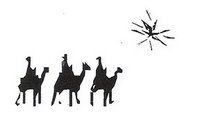
\includegraphics[height=3cm]{images/3kings_star.png}\hfill\mbox{}

